\documentclass[11pt]{article}

\usepackage[T1]{fontenc}
\usepackage[utf8]{inputenc}
\usepackage{lmodern}
\usepackage{microtype}
\usepackage[a4paper,margin=2.4cm]{geometry}
\usepackage{amsmath,amssymb}
\usepackage{booktabs}
\usepackage{threeparttable}
\usepackage{tabularx}
\usepackage{multirow}
\usepackage{graphicx}
\usepackage[section]{placeins}
\usepackage{enumitem}
\usepackage{xcolor}
\usepackage{hyperref}
\usepackage[nameinlink,noabbrev]{cleveref}

\hypersetup{
  colorlinks=true,
  linkcolor=blue!55!black,
  citecolor=blue!55!black,
  urlcolor=blue!55!black
}
\setlength{\parindent}{1.5em}
\setlength{\parskip}{0.2em}
\newcommand{\method}[1]{\textsc{#1}}
\newcommand{\todo}[1]{\textcolor{red!70!black}{[Administrative item: #1]}}

\title{Text-First Hierarchical Retrieval for Auditable Pharmaceutical Regulatory Evidence and Supply-Chain Fact Verification}
\author{
  Kaifeng Sun\\
  China Jiliang University, Hangzhou, China\\
  \texttt{2300702216@cjlu.edu.cn}
}
\date{}

\begin{document}
\maketitle

\begin{abstract}
Pharmaceutical analysts must recover citable regulatory passages while checking structured facts about products, ingredients, manufacturers, and shortages. We present a text-first framework that preserves this evidential distinction. It parses 32 documents into 2,478 source chunks and 312 tables, retains document hierarchy, and links the corpus to a provenance-bearing graph with 7,578 nodes and 15,237 edges. Two independent reviewers labelled a method-blinded 60-question pool; core binary evidence agreement was 0.941 ($\kappa=0.792$, AC1$=0.918$). After adjudication and two prespecified exclusions, BM25 achieved Hit@5 of 0.948, MRR of 0.820, and nDCG@5 of 0.800 on 58 questions. A locked Qwen3 reranker raised the point estimates to 0.983, 0.832, and 0.817, although paired intervals did not establish a general gain. A feedback-motivated zero-shot MedCPT experiment performed substantially worse. Graph access did not improve text ranking, but a separate exploratory test on 28 audit-qualified, relation-derived questions found that relation-aware ranking recovered the exact evidence chain within five candidates for 0.786 of questions. These findings support a bounded architecture: lexical retrieval ranks passages, hierarchy supplies context, neural models require corpus-specific validation, and graph chains verify structured claims without replacing source text.
\end{abstract}

\noindent\textbf{Keywords:} pharmaceutical regulation; evidence retrieval; knowledge graph; drug shortages; hierarchical retrieval; neural reranking; provenance

\section{Introduction}
\label{sec:introduction}

Manufacturing failures, constrained inputs, discontinuations, demand shocks, and slow recovery can all contribute to drug shortages. FDA analyses emphasize quality problems, limited capacity, and small supplier bases \cite{fda2019shortages}. A public shortage record may identify a presentation, company, availability state, and reported reason, but analysts must consult separate regulatory sources to interpret quality risk, supplier control, or change management.

Those sources are difficult retrieval targets. A short clause may inherit scope from several parent headings, and PDF conversion can separate a table value from its conditions. Guideline numbers, defined phrases, and product identifiers often carry more evidential weight than broad semantic similarity. Structured facts create another requirement: NDCs, manufacturers, active ingredients, and events form relations, not citable prose. Treating a graph edge as a quotation or a similar passage as a database fact obscures provenance.

We address this problem as evidence retrieval rather than answer generation. The framework returns source passages with hierarchy and separately returns provenance-bearing graph paths. It compares lexical, dense, enriched, hierarchical, fused, and neural rankings under frozen evaluation protocols. The final evidence set was independently labelled by the author and a domain reviewer, jointly adjudicated, and executed once after method locking.

The contribution is empirical as well as architectural. We test where hierarchy and graphs help, where they do not, and whether a biomedical retrieval model transfers to pharmaceutical regulation. The system does not predict shortage duration or patient harm. It exposes what a frozen source says and how a structured record connects named entities.

\section{Related Work}
\label{sec:related}

\subsection{Pharmaceutical regulatory evidence and shortages}

The FDA Drug Shortages Task Force identified weak incentives for low-margin products, limited market recognition of mature quality systems, and logistical and regulatory barriers to recovery as recurring root causes \cite{fda2019shortages}. FDA shortage records use defined categories that include current good manufacturing practice requirements, regulatory delay, active- or inactive-ingredient shortage, discontinuation, shipping delay, and increased demand \cite{fdaShortageFAQ}. The openFDA interface publishes machine-readable shortage fields and harmonized identifiers, which support reproducible collection but do not turn database fields into regulatory conclusions \cite{openfdaShortages}. FDA's draft risk-management-plan guidance links proactive supply-risk identification to ICH Q9 principles, while explicitly retaining draft status \cite{fdaShortageRMP2022,ichQ9R1}.

Regulatory evidence is distributed across authorities, document families, and lifecycle stages. ICH Q10 treats knowledge management and quality risk management as enablers throughout the product lifecycle \cite{ichQ10}. FDA's quality-systems guidance explains how a modern quality system can operate consistently with current good manufacturing practice \cite{fdaQualitySystems2006}. Annex 11 adds computerized-system lifecycle controls \cite{ecAnnex11}. Our system preserves the authority, document, section, and source location of each passage because a retrieved statement must remain distinguishable from a generated summary or a graph relation.

Recent domain studies provide close precedents. Gray et al. classified free regulatory text into standard labeling sections \cite{gray2023regulatory}. Saraswat et al. evaluated question similarity for pharmaceutical regulatory search using expert-annotated entailment pairs \cite{saraswat2023regulatory}. Proestel et al. studied semantic search over FDA guidance, and Nanua et al. evaluated RAG against laboratory regulations \cite{proestel2025semantic,nanua2025raven}. These studies support the practical relevance of regulatory retrieval. Our evaluation differs by separating source-chunk ranking from structured shortage-path recovery and by testing whether added semantic and graph components improve retrieval on a fixed corpus.

\subsection{Lexical, dense, and neural retrieval}

BM25 derives a probabilistic lexical score from term frequency, inverse document frequency, and length normalization \cite{robertson2009bm25}. Dense passage retrieval instead learns query and passage encoders whose vectors can be searched efficiently \cite{karpukhin2020dpr}. The two approaches respond to different signals. A dense model can bridge paraphrases, while a lexical model can exploit exact guideline numbers, table labels, product terms, and defined phrases. Our experiments therefore treat BM25 as a full baseline rather than a preliminary component that semantic retrieval is assumed to surpass.

HyDE addresses zero-shot dense retrieval by generating a hypothetical document for a query and using its embedding to locate real passages \cite{gao2023hyde}. We adapt the same general idea on the index side: generated questions and summaries point back to source chunks and never count as evidence. Youtu-Embedding, the frozen dense encoder used in our experiments, was trained through a framework designed to balance information retrieval and semantic textual similarity objectives \cite{zhang2025codiemb}. We evaluate the resulting representations in this corpus rather than transferring benchmark claims to pharmaceutical text.

Neural rerankers apply richer query-document interaction after a first-stage retriever has reduced the candidate set. Sequence-to-sequence rerankers can interpret relevance-label token probabilities as ranking scores \cite{nogueira2020monot5}; multilingual long-context rerankers extend this pattern beyond short English passages \cite{zhang2024mgte}. Qwen3-Reranker provides generative rerankers at several parameter scales \cite{zhang2025qwen3embedding}. We use its 0.6B variant only in a locked supplementary analysis over BM25's top 50. This design tests candidate reordering without allowing the reranker to recover a source chunk that BM25 failed to retrieve.

\subsection{Hierarchical and graph-based retrieval}

RAPTOR recursively embeds, clusters, and summarizes text into a retrieval tree to expose multiple levels of abstraction \cite{sarthi2024raptor}. GraphRAG extracts entity graphs and community summaries to answer corpus-level questions \cite{edge2024graphrag}. Those objectives differ from exact regulatory passage retrieval. A community summary may help explain a corpus but cannot replace the source clause used to justify a regulated decision.

Knowledge graphs provide explicit entities, relations, identity choices, schemas, and provenance \cite{hogan2021knowledgegraphs}. We use these properties to represent shortage events and document structure. We do not assume that graph connectivity is equivalent to textual relevance. Reciprocal rank fusion (RRF) offers a score-scale-independent way to combine rankings \cite{cormack2009rrf}; our experiments include both unconditional RRF and constrained variants so that a failed fusion remains visible rather than being removed after inspection.

\section{Task Definition}
\label{sec:task}

Each document is parsed into an ordered tree of headings, sections, source chunks, and tables. Let $C$ denote the source chunks and $\mathcal{G}=(V,E,\tau_V,\tau_E)$ the typed evidence graph.

For a natural-language query $q$, the text task returns a ranking
\begin{equation}
R_C(q)=(c_1,c_2,\ldots), \qquad c_i\in C.
\end{equation}
Only source chunks confirmed by human reviewers, denoted $C_q^*$, count as relevant. A generated question, section summary, table summary, document node, or shortage entity cannot satisfy a text Gold judgment.

The structured task returns paths
\begin{equation}
P_G(q)=\{p_1,p_2,\ldots\}, \qquad p_i=(v_1,e_1,v_2,\ldots,v_k),
\end{equation}
with edge direction and source metadata preserved. A path succeeds when an accepted node and edge sequence appears in the first $K$ candidates. Structured nodes never enter text Hit@$K$, reciprocal rank, or nDCG.

The interface may display a passage and a path together, but their evidential roles remain explicit. \Cref{fig:dual-path} summarizes how an analyst request invokes text retrieval, structured relation-chain retrieval, or both while preserving this distinction.

\begin{figure}[!t]
  \centering
  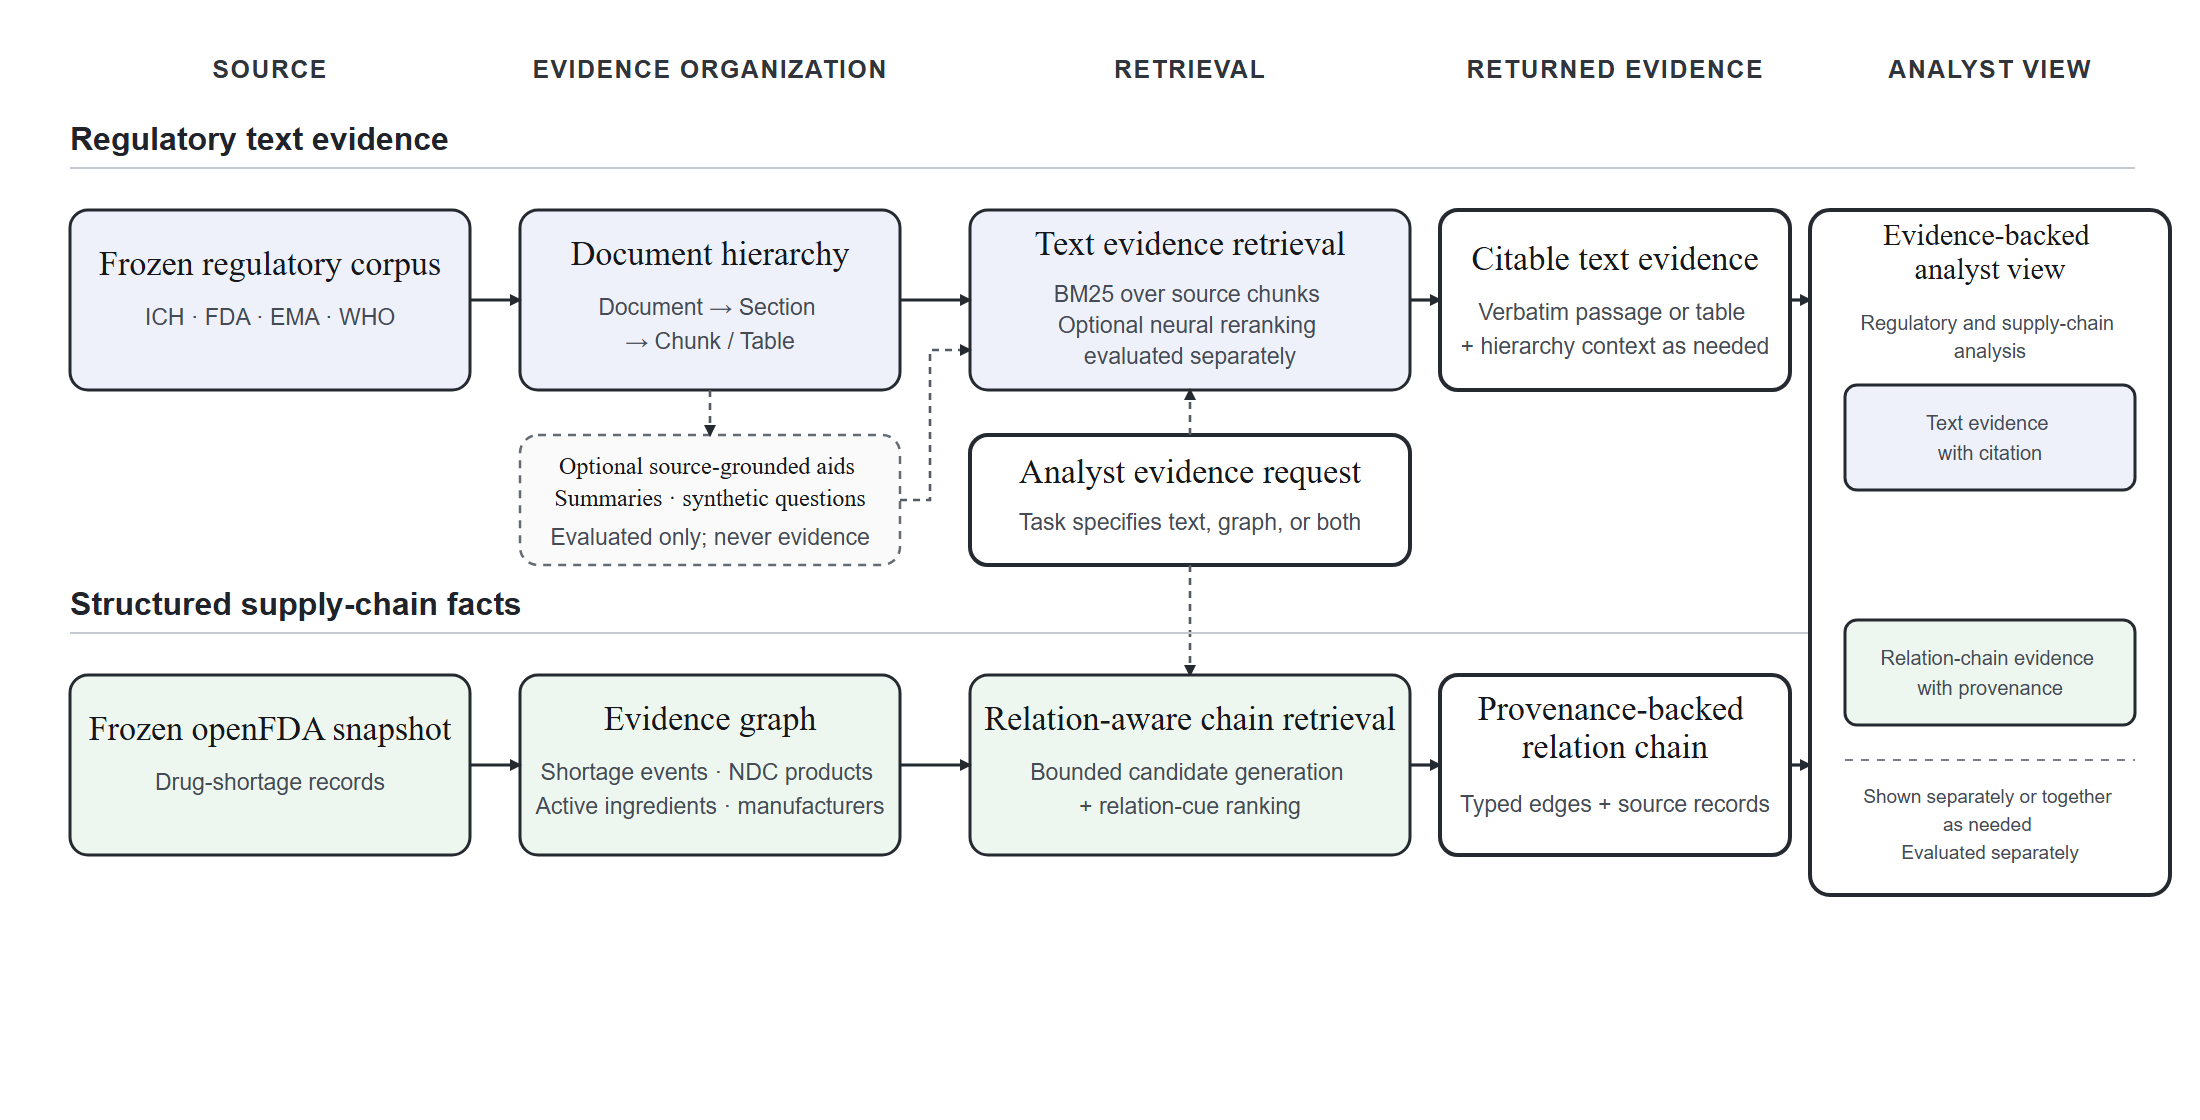
\includegraphics[width=\linewidth]{figures/dual_path_framework.png}
  \caption{Overview of the proposed dual-path auditable evidence retrieval framework. Analyst requests may invoke text retrieval, structured relation-chain retrieval, or both. Source-grounded summaries and synthetic questions were evaluated as optional retrieval aids but never treated as evidence; returned evidence remains a citable source passage, table, or provenance-bearing graph record.}
  \label{fig:dual-path}
\end{figure}

\section{Corpus and Evidence Graph}
\label{sec:data}

\subsection{Regulatory corpus}

The frozen corpus contains 32 English regulatory and technical documents. It covers multiple ICH Q1--Q14 quality guidelines and drafts, ICH M7(R2), European GMP Annex 11, FDA guidance on pharmaceutical quality systems, and WHO material on essential medicines and stability. PDF-to-Markdown conversion, structural parsing, and cleaning produced 2,478 non-empty source chunks with a maximum length of 2,271 characters. The parser identified 312 table records. \Cref{tab:corpus} summarizes the frozen resources.

\begin{table}[t]
\centering
\begin{threeparttable}
\caption{Frozen corpus and evidence-graph statistics.}
\label{tab:corpus}
\begin{tabular}{lr}
\toprule
Resource & Count \\
\midrule
Regulatory and technical documents & 32 \\
Source chunks & 2,478 \\
Table records & 312 \\
Source-constrained hypothetical questions & 3,917 \\
Section summaries & 221 \\
Document summaries & 32 \\
Graph nodes & 7,578 \\
Graph edges & 15,237 \\
Shortage events & 1,633 \\
NDC product nodes & 1,593 \\
Active-ingredient nodes & 225 \\
Manufacturer nodes & 131 \\
\bottomrule
\end{tabular}
\begin{tablenotes}[flushleft]\footnotesize
\item Counts come from the frozen enrichment and graph-build manifests. Generated questions and summaries are index-side aids and never count as Gold evidence.
\end{tablenotes}
\end{threeparttable}
\end{table}


The parser retained heading levels, parent-child relations, and local order. The graph contains 756 \texttt{PARENT\_OF} edges and 2,446 \texttt{NEXT} edges. It also contains summaries for 221 section nodes and 32 document nodes. Each summary points to the source unit through \texttt{SUMMARIZES}. Summaries can support routing and browsing, but the evaluation never treats them as source evidence.

\subsection{Source-constrained enrichment}

The enrichment pipeline generated hypothetical questions for eligible chunks of at least 100 characters. A 500-character threshold selected one of two context strategies. Longer chunks relied mainly on their own text; shorter chunks also received parent headings, neighboring text, and same-section table context to restore omitted scope. The frozen corpus contains 3,917 generated question profiles that passed structural and source-grounding checks. The pipeline also created short chunk summaries for eligible long passages and 311 table summaries.

All generated representations map to a source chunk. A retrieved profile is resolved to that chunk before deduplication and evaluation. This rule prevents a plausible generated statement from becoming evidence merely because it resembles the question.

\subsection{Structured shortage data and graph schema}

Structured records came from an openFDA drug-shortage snapshot frozen on 10 July 2026 \cite{openfdaShortages}. The pipeline normalized generic names, company names, package NDCs, availability states, reported reasons, status fields, and update dates into shortage-event, NDC-product, active-ingredient, and manufacturer nodes. Every normalized record retains a pointer to its raw snapshot entry.

The resulting graph contains 7,578 nodes and 15,237 edges. Its major node classes include 2,478 source chunks, 1,633 shortage events, 1,593 NDC products, 225 active ingredients, 131 manufacturers, 32 regulatory documents, 312 tables, 221 section summaries, and 32 document summaries. Supply facts use relations such as \texttt{AFFECTS\_NDC\_PRODUCT}, \texttt{HAS\_ACTIVE\_INGREDIENT}, and \texttt{REPORTED\_BY}. Document structure uses \texttt{CONTAINS}, \texttt{PARENT\_OF}, \texttt{NEXT}, \texttt{HAS\_TABLE}, and \texttt{SUMMARIZES}. Cross-document relations such as \texttt{REFERENCES}, \texttt{SUPERSEDES}, \texttt{COMPLEMENTS}, and \texttt{INTERPRETS} require an explicit source citation or a confirmed rule.

The schema uses conservative semantics. \texttt{MENTIONS} records a normalized alias match and does not imply causation or regulatory dependence. \texttt{REFERENCES} records an explicit citation and does not imply that one document governs another. Uncertain identity links remain \texttt{SAME\_AS\_CANDIDATE} rather than forcing a manufacturer or product merge.

\section{Methods}
\label{sec:methods}

\subsection{Bottom-up source-chunk retrieval}

The bottom-up path searches an index of source-linked representations. The frozen dense encoder is \texttt{tencent/Youtu-Embedding}, used without task-specific fine-tuning. An auxiliary summary or hypothetical question that matches the query is immediately mapped back to its source chunk; duplicate chunks retain their best rank. FAISS performs vector search. The source chunk, not the generated representation, is returned to the reviewer.

The lexical baseline applies BM25 to a common payload consisting of parent context, heading text, and the first 2,000 characters of the source chunk. Tokenization lowercases alphanumeric terms. The fixed parameters are $k_1=1.2$ and $b=0.75$ \cite{robertson2009bm25}. Dense and lexical methods use the same 2,478 source identifiers.

\subsection{Top-down document routing}

The top-down path first retrieves from an index containing source representations and generated question profiles. Candidate ranks vote for documents using reciprocal-rank contributions. The two highest-scoring documents define a restricted search space. The system then returns to the source-chunk index, ranks chunks within those documents, and exposes the path from the document root through the parent section to each candidate. Direct children of a routed section can enter the candidate set with lower weight.

This path uses generated questions to decide where to search, not what to cite. The final ranking contains only source chunks. The design resembles hierarchical retrieval in its use of multiple levels, while retaining the original document tree instead of building a learned clustering tree \cite{sarthi2024raptor}.

\subsection{Bounded graph traversal}

The graph engine produces two outputs. Structured paths start from recognized shortage events, NDCs, active ingredients, products, or manufacturers and preserve relation direction and provenance. Experimental graph-constrained text paths start from a document or topic anchor, traverse a bounded neighborhood, and use the reachable documents as a filter before ranking source chunks.

Traversal uses a deterministic bounded breadth-first search. The formal configuration limits path depth to four, expands at most 800 states per query, and caps neighbors per node. For an NDC- or shortage-specific question, the system can return a path of the form shortage event $\rightarrow$ NDC product $\rightarrow$ active ingredient together with manufacturer, availability, reason, and update fields. These records remain outside the text ranking.

\subsection{Fusion and adaptive variants}

Bottom-up, top-down, and graph-constrained text rankings can be fused by RRF \cite{cormack2009rrf}. For source chunk $c$,
\begin{equation}
s_{\mathrm{RRF}}(c)=\sum_{r\in\{b,t,g\}}\frac{w_r}{k_0+\operatorname{rank}_r(c)},
\end{equation}
where $k_0=60$, $w_b=w_t=1$, and $w_g=0.5$ when graph gating is active. The graph gate requires a direct structured record, an explicit regulatory-document anchor, or agreement between graph-reachable documents and the text routes. Otherwise $w_g=0$.

The adaptive method adds bounded metadata gains for explicit document matches and table intent. The gains rerank only existing source candidates. We report the unconditional and adaptive variants because a gate that sounds plausible can still damage ranking.

\subsection{BM25-anchored selective reranking}

The first selective reranker combines source-level BM25 and dense ranks. It returns BM25 unchanged unless the query has explicit table intent or the union of the two top-five lists contains at least two distinct table chunks. When enabled, it assigns
\begin{equation}
s(c)=\frac{1}{60+r_{\mathrm{BM25}}(c)}+\frac{1}{60+r_{\mathrm{dense}}(c)}+\frac{0.25I_{\mathrm{table}}(c)}{61}.
\end{equation}
Missing ranks contribute zero. Ties resolve by BM25 rank, dense rank, and chunk identifier. The gate depth, support threshold, and table weight were selected on 90 observed queries and then frozen.

After the 58-query adjudicated evaluation, we added one supplementary post hoc neural condition to address whether a modern cross-encoder-style reranker could improve ordering inside a strong lexical candidate set. Qwen3-Reranker-0.6B reranks the fixed BM25 top 50 with the instruction ``Given a pharmaceutical regulatory question, retrieve a source passage that directly supports the answer.'' The model uses BF16, a maximum sequence length of 1,024 tokens, batch size eight, deterministic inference, and normalized probabilities of the official \texttt{yes}/\texttt{no} relevance tokens \cite{zhang2025qwen3embedding}. The model, code, candidates, corpus, Gold package, and settings were hashed and committed before any formal score was inspected. Because the same adjudicated queries had already been used to compare earlier methods, this analysis is supplementary and post hoc rather than confirmatory.

\section{Experimental Design}
\label{sec:experiments}

\subsection{Research questions}

The experiments address seven questions. RQ1 measures bottom-up, top-down, and fused text retrieval. RQ2 tests unconditional and gated graph access for source-chunk ranking. RQ3 asks whether the graph can recover six manually accepted shortage-event paths. RQ4 compares BM25 with dense retrieval and cumulative index-side enrichment. RQ5 tests a source-level selective table gate on a new confirmation set. RQ6 repeats that comparison on a new, independently double-annotated and jointly adjudicated pool. RQ7, added after RQ6, asks whether a locked modern reranker can improve ordering within BM25's top 50. RQ7 is labelled supplementary and post hoc throughout.

We did not reproduce NaiveRAG, GraphRAG-Global, LightRAG, HippoRAG, or proprietary systems. We also did not compare graph traversal against direct openFDA queries or relational joins. The study therefore makes no cross-system state-of-the-art claim.

\subsection{Development, holdout, and confirmation sets}

The initial 60-query development set informed retrieval rules. A separate 30-query principal holdout covered 10 single-clause, six table, four document-structure, four cross-document, and six supply-chain-path questions. The methods and Gold evidence were frozen before the holdout run. The path questions required both structured nodes and regulatory chunks; only chunks entered text metrics.

RQ4 used a different 30-query ablation set: 10 single-clause, eight table, six document-structure, and six cross-document questions. The questions were written from previously unused frozen passages and tables without consulting retrieval rankings. Twenty-two were confirmed in the first review; eight were narrowed and confirmed in a second round. Its Gold chunks do not overlap the earlier development or principal-holdout Gold sets. Once RQ4 motivated a table gate, this set became observed development data.

RQ5 combined 90 observed queries for parameter selection, then evaluated the frozen gate on another 30-query confirmation set. Candidate passages were shuffled and the review workbook hid method names, scores, ranks, and true chunk identifiers. Twenty-four questions were confirmed directly; six were narrowed and confirmed in a second pass. ``Method blinded'' refers to the review interface, not to double-blind study conduct.

\subsection{Independent annotation and adjudication}

RQ6 introduced 60 new questions: 20 single-clause, 15 table, 15 document-structure, and 10 cross-document questions. Normalized question strings were deduplicated against all prior pools. Each question received 8--12 candidate passages drawn from source anchors, BM25, the raw dense index, hierarchical routing, and same-document hard negatives. The workbook concealed the candidate source, method, score, rank, chunk identifier, and source-anchor identity.

Reviewer A was the author. Reviewer B had pharmaceutical, manufacturing, medical, and regulatory expertise. Both reviewed the same passages in separately randomized orders and did not compare labels before submission. Question labels were \texttt{Answerable}, \texttt{Needs Revision}, or \texttt{Invalid}; evidence-completeness labels were \texttt{Complete}, \texttt{Incomplete}, or \texttt{Unclear}. Passage labels were \texttt{Sufficient}, \texttt{Required Component}, \texttt{Context Only}, \texttt{Not Supporting}, or \texttt{Unclear}. The first two passage labels form the core binary Gold set used for retrieval metrics.

The original labels remain unchanged in the audit archive. Joint adjudication addressed question-status differences, core Gold disagreements, and missed labels. Two table questions ended with incomplete evidence and were retained in the audit ledger but excluded under the prespecified rule. The formal run therefore contained 58 questions and no unresolved judgments.

\subsection{Methods and metrics}

The principal holdout compares bottom-up dense retrieval, top-down routing, graph-constrained text retrieval, text-only RRF, unconditional three-path RRF, and adaptive variants. RQ4 compares BM25 with four cumulative dense indexes: R1 contains source chunks; R2 adds chunk summaries; R3 adds 3,917 generated question profiles; and R4 adds 311 table-summary profiles. BM25+R4 uses equal-weight RRF. RQ5 and RQ6 compare context-matched BM25, R1, unconditional source-level RRF, and the selective table gate. RQ7 compares the same BM25 top-50 ranking with its Qwen3 reranking.

Text metrics are Hit@1, Hit@3, Hit@5, reciprocal rank, and binary nDCG@5; RQ7 also reports Hit@50 and MRR@50. nDCG rewards relevant chunks near the top of a ranking \cite{jarvelin2002ndcg}. Structured-path recovery uses success@5 and remains separate from text metrics.

Confidence intervals use 10,000 query-level bootstrap samples. Paired Hit@5 comparisons use McNemar's exact test \cite{mcnemar1947correlated}; MRR and nDCG@5 use the paired Wilcoxon signed-rank test \cite{wilcoxon1945rank}. Holm's procedure controls the familywise error rate across each three-metric comparison family \cite{holm1979multiple}. RQ5's prespecified primary outcome was the selective gate's MRR difference from BM25. Success required a difference of at least 0.03, a bootstrap lower bound above zero, Holm-adjusted $p<0.05$, and no Hit@5 decrease greater than 0.033.

Inter-reviewer reporting includes exact agreement, Cohen's $\kappa$ \cite{cohen1960kappa}, and Gwet's AC1 \cite{gwet2008ac1}. Core Gold agreement also includes positive agreement, macro Jaccard, and macro F1. Query-cluster bootstrap intervals preserve within-query passage dependence.

\section{Results}
\label{sec:results}

\subsection{Historical holdout and initial graph feasibility}

On the 30-question principal holdout, top-down routing reached Hit@5 of 0.767 versus 0.700 for bottom-up dense retrieval. The adaptive method also reached 0.767, but its paired interval against text-only fusion included zero. Graph-constrained text retrieval reached only 0.100, and disabling graph access left adaptive aggregate metrics unchanged.

The graph recovered all six accepted shortage-event paths within five candidates. Text retrieval answered only one of their six accompanying regulatory targets within five. This initial result supported explicit-relation feasibility and motivated a more controlled chain-ranking test.

\subsection{Enrichment ablation}

BM25 led the independent enrichment ablation with Hit@5 of 0.867, MRR of 0.726, and nDCG@5 of 0.662 (\Cref{tab:ablation}). Adding chunk summaries changed little. Generated question profiles reduced MRR by 0.171 and nDCG@5 by 0.167 versus the raw dense index; both paired adjusted tests gave $p=0.024$. Mapping generated items back to source chunks preserved provenance but did not prevent competition for nearest-neighbor positions.

\subsection{Adjudicated evaluation}

The reviewers agreed on 96.7\% of question-status and evidence-completeness labels. Core binary passage agreement was 0.941, with $\kappa=0.792$ (95\% interval [0.718, 0.862]) and AC1$=0.918$ ([0.880, 0.949]). Joint adjudication left no unresolved item.

On the one-shot 58-question run, BM25 achieved Hit@5 of 0.948, MRR of 0.820, and nDCG@5 of 0.800. The selective gate reached 0.897, 0.787, and 0.757, failing its prespecified superiority rule.

\begin{table}[t]
\centering
\begin{threeparttable}
\caption{Independent enrichment ablation ($n=30$; query-bootstrap 95\% confidence intervals).}
\label{tab:ablation}
\small
\begin{tabularx}{\textwidth}{l*{3}{>{\centering\arraybackslash}X}}
\toprule
Method & Hit@5 & MRR & nDCG@5 \\
\midrule
BM25 raw & \textbf{0.867 [0.733, 0.967]} & \textbf{0.726 [0.593, 0.846]} & \textbf{0.662 [0.528, 0.789]} \\
R1: source chunks & 0.733 [0.567, 0.900] & 0.557 [0.412, 0.702] & 0.526 [0.380, 0.673] \\
R2: R1 + chunk summaries & 0.733 [0.567, 0.867] & 0.554 [0.408, 0.703] & 0.524 [0.380, 0.669] \\
R3: R2 + generated questions & 0.567 [0.400, 0.733] & 0.384 [0.253, 0.522] & 0.357 [0.220, 0.502] \\
R4: R3 + table summaries & 0.567 [0.400, 0.733] & 0.384 [0.252, 0.524] & 0.357 [0.217, 0.500] \\
BM25 + R4 RRF & 0.733 [0.567, 0.867] & 0.606 [0.461, 0.747] & 0.508 [0.366, 0.652] \\
Full adaptive & 0.800 [0.667, 0.933] & 0.608 [0.464, 0.747] & 0.571 [0.430, 0.713] \\
\bottomrule
\end{tabularx}
\begin{tablenotes}[flushleft]\footnotesize
\item R1--R4 are cumulative flat dense indexes. Generated representations map back to source chunks before evaluation.
\end{tablenotes}
\end{threeparttable}
\end{table}


\subsection{Neural boundary experiments}

BM25 found Gold within its top 50 for all 58 questions. Qwen3 reranking raised Hit@5 to 0.983, MRR to 0.832, and nDCG@5 to 0.817. The paired differences were 0.034 [0.000, 0.086], 0.012 [-0.082, 0.104], and 0.017 [-0.058, 0.093], respectively. The point estimates improved, but the intervals did not establish a general gain.

MedCPT gave the opposite result. Full-corpus dual-encoder retrieval reached Hit@5 of 0.345, MRR of 0.300, and nDCG@5 of 0.246. MedCPT cross-encoding of BM25's top 50 preserved candidate recall but reduced the three metrics to 0.603, 0.457, and 0.431. All paired 95\% intervals against BM25 were below zero for these metrics. The pattern held across single-clause, table, document-structure, and cross-document slices.

\begin{table}[t]
\centering
\begin{threeparttable}
\caption{Source-chunk retrieval on 58 adjudicated questions.}
\label{tab:final58}
\begin{tabular}{lccc}
\toprule
Method & Hit@5 & MRR & nDCG@5 \\
\midrule
Context-matched BM25 & 0.948 & 0.820 & 0.800 \\
Youtu source-chunk dense & 0.759 & 0.574 & 0.545 \\
Selective table gate & 0.897 & 0.787 & 0.757 \\
Qwen3 over BM25 top 50$^{*}$ & \textbf{0.983} & \textbf{0.832} & \textbf{0.817} \\
MedCPT dual encoder$^{*}$ & 0.345 & 0.300 & 0.246 \\
MedCPT over BM25 top 50$^{*}$ & 0.603 & 0.457 & 0.431 \\
\bottomrule
\end{tabular}
\begin{tablenotes}[flushleft]\footnotesize
\item $^{*}$Feedback-motivated locked extensions on already observed Gold questions. Qwen3 and the MedCPT cross-encoder rerank BM25's frozen top 50; MedCPT dual-encoder retrieval searches all 2,478 chunks.
\end{tablenotes}
\end{threeparttable}
\end{table}


\subsection{Exploratory evidence-chain ranking}

Candidate generation contained the accepted chain for every question. On the 28 audit-qualified questions, R1 achieved exact-chain Hit@1 of 0.571, Hit@3 and Hit@5 of 0.786, and MRR of 0.663 (\Cref{tab:graphchain}). Its Hit@5 difference from M0 was 0.643 [0.464, 0.821]. Removing relation cues reduced Hit@5 to 0.143, whereas removing orientation reduced it to 0.750; the R1--direction-off difference was 0.036 [-0.071, 0.143]. Thus most measured gain came from matching relation phrases rather than the orientation term.

Performance varied sharply by task. R1 recovered all shortage chains within one candidate and reached Hit@5 of 0.900 on regulatory logic, but only 0.375 on the eight retained API-supply questions. The transparent 30-question analysis, which includes the two ambiguous questions, gave Hit@5 of 0.733 and MRR of 0.626. Twelve queries reached the deterministic 50,000-candidate cap, but none aborted or lacked an anchor.

\begin{table}[!ht]
\centering
\begin{threeparttable}
\caption{Exact evidence-chain ranking on 28 audit-qualified questions.}
\label{tab:graphchain}
\small
\begin{tabular}{lcccc}
\toprule
Method & Hit@1 & Hit@3 & Hit@5 & MRR \\
\midrule
B0: untyped traversal & 0.000 & 0.036 & 0.179 & 0.067 \\
M0: relation-blind matched & 0.036 & 0.107 & 0.143 & 0.140 \\
Cue-off & 0.036 & 0.071 & 0.143 & 0.180 \\
Direction-off & 0.500 & 0.714 & 0.750 & 0.600 \\
R1: relation-aware & \textbf{0.571} & \textbf{0.786} & \textbf{0.786} & \textbf{0.663} \\
\bottomrule
\end{tabular}
\begin{tablenotes}[flushleft]\footnotesize
\item Questions were constructed from known graph relations. Two ambiguous API questions were retained in the audit ledger but excluded from strict metrics; the unfiltered 30-question R1 Hit@5 was 0.733.
\end{tablenotes}
\end{threeparttable}
\end{table}


\Cref{fig:retrieval-findings} consolidates the principal text-retrieval boundary, graph-chain ablation, and task-specific failure pattern in a common Hit@5 view.

\begin{figure}[!t]
  \centering
  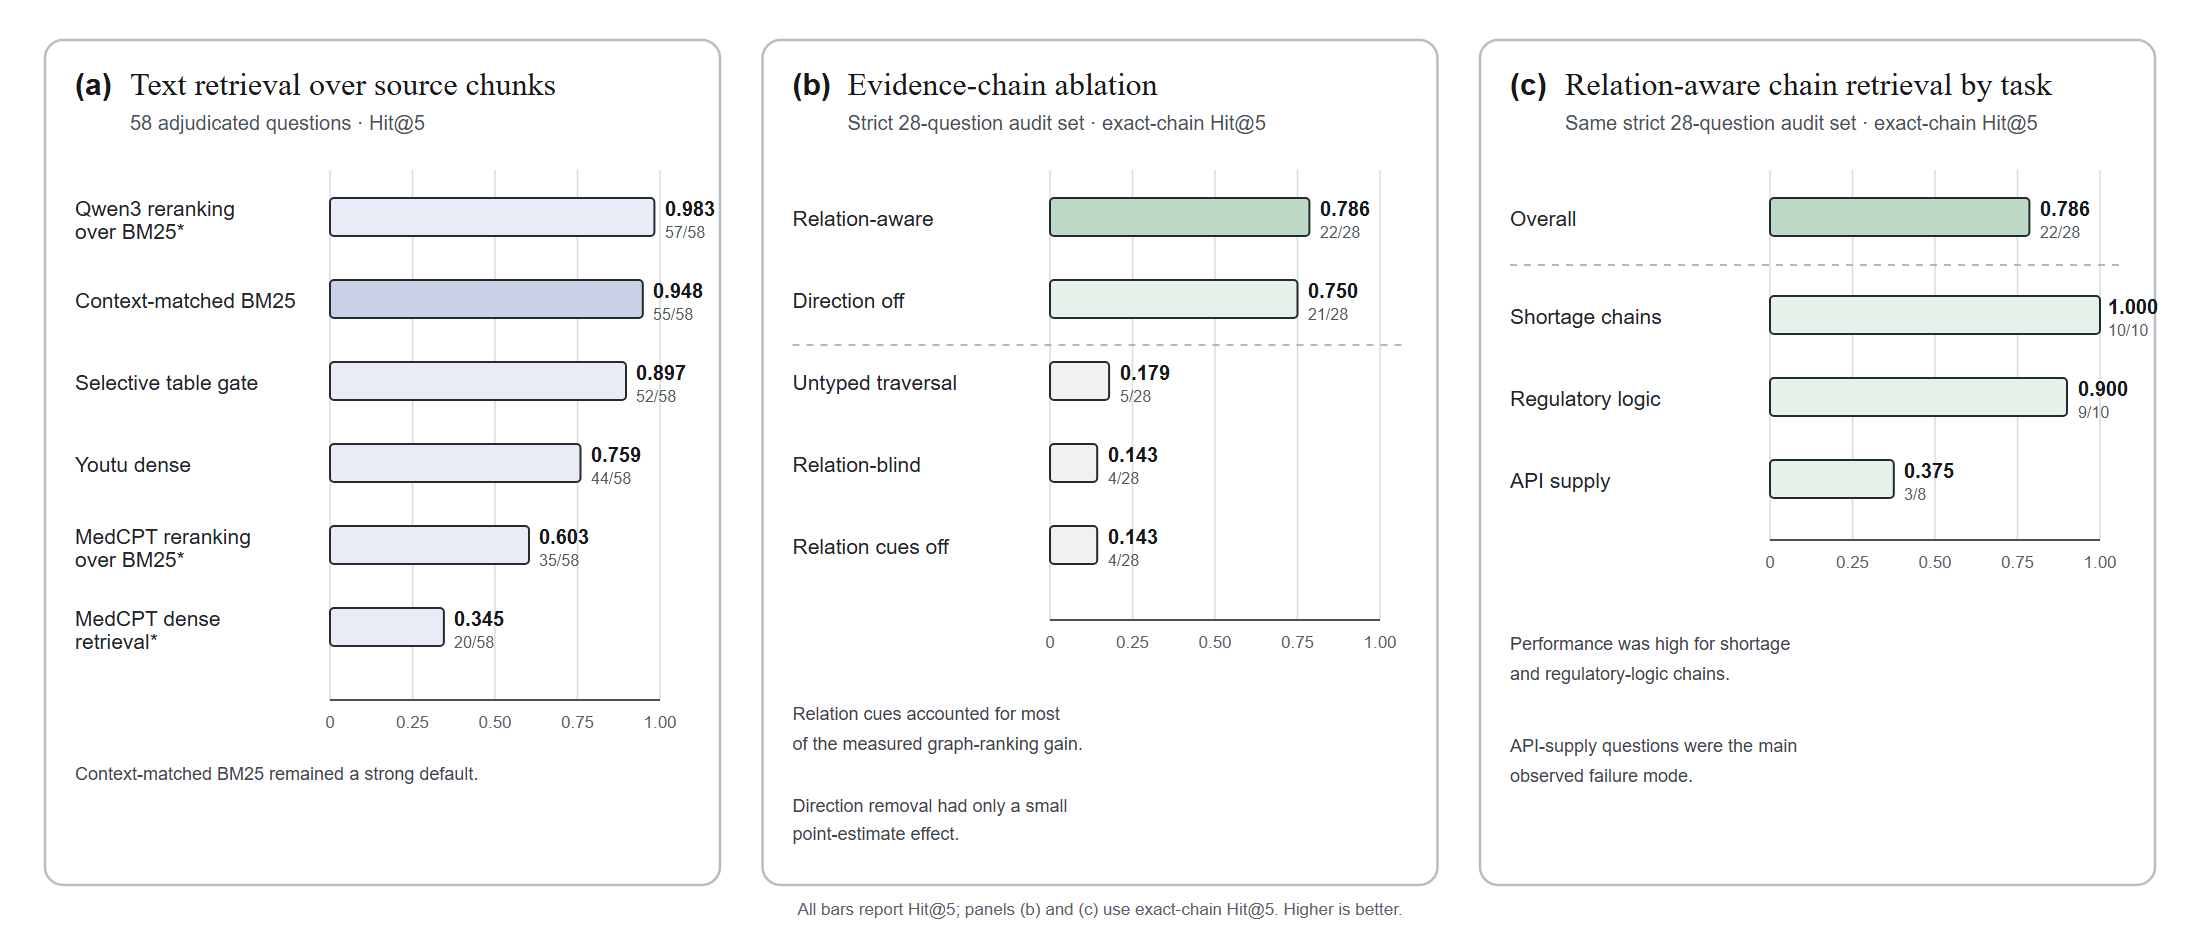
\includegraphics[width=\linewidth]{figures/retrieval_findings_summary.png}
  \caption{Summary of source-chunk and evidence-chain retrieval results. (a) Hit@5 on 58 adjudicated text questions. Asterisks mark feedback-motivated post hoc extensions evaluated under subsequently locked, unchanged inference protocols after the Gold set had been observed; they are interpreted as boundary analyses. The 95\% paired-bootstrap interval for the Qwen3--BM25 Hit@5 difference included zero. The darker lavender fill identifies the primary BM25 baseline. (b) Exploratory exact-chain Hit@5 for the relation-aware method and its controls on the strict 28-question audit set. (c) Exploratory exact-chain Hit@5 for the complete relation-aware method by task. Two questions with non-unique frozen-graph paths were retained in the 30-question audit record but excluded from strict exact-chain evaluation. Values show proportions and exact hit counts.}
  \label{fig:retrieval-findings}
\end{figure}

\section{Discussion}
\label{sec:discussion}

\subsection{A text-first division of labor}

Exact guideline numbers, table labels, defined terms, and clause wording gave BM25 a strong advantage. Flat generated profiles displaced source candidates, and equal-weight fusion diluted lexical hits. Qwen3 recovered two additional Top-5 successes but did not establish a general paired gain. MedCPT performed worse despite biomedical retrieval pretraining, especially on single-clause questions. PubMed article relevance and regulatory clause entailment are different tasks.

The evidence supports lexical first-stage retrieval with optional, separately validated neural reordering. Hierarchy still adds parent sections, siblings, and table membership to each result. These navigation gains do not require summaries to count as evidence.

\subsection{What the graph contributes}

Graph topology did not improve passage ranking because \texttt{CONTAINS}, \texttt{NEXT}, or \texttt{REFERENCES} does not prove relevance. Shortage paths answer a different question: which record names the event, NDC, ingredient, company, status, and reason. Such a path supports provenance, not causation. The six accepted paths establish feasibility only; direct database joins, path precision, abstention, entity linking, and temporal invalidation remain to be tested.

\subsection{Implications for regulatory retrieval evaluation}

A favorable table slice motivated a selective gate, but two later sets failed to confirm it. This sequence guards against promoting a local pattern to a general claim. Independent review also showed stronger agreement for binary evidence membership than for five-way evidence roles, supporting binary Gold for ranking while retaining richer labels for audit.

\subsection{Limitations}

The final set contains 58 questions, and slice estimates remain unstable. One reviewer was the author and the other was a single external expert. Source-derived questions may retain identifiers that favor BM25; future evaluators should write independent information needs.

The corpus contains 32 selected English documents and one frozen US shortage snapshot. It does not cover all jurisdictions or regulatory versions. The 10 July 2026 shortage state is historical, and the graph lacks tested temporal invalidation. MedCPT and Qwen3 were zero-shot single-model comparisons, not domain fine-tuning studies.

We evaluated retrieval and path recovery rather than answer correctness, hallucination, latency, or analyst utility. A larger answer-level blinded study must test whether separating text and graph evidence improves decisions.

\section{Conclusion}
\label{sec:conclusion}

This study examined two evidence tasks that a pharmaceutical decision-support system should not collapse: retrieval of citable regulatory passages and verification of structured drug-shortage facts. We built a hierarchical corpus with source-preserving summaries and tables, connected it to a provenance-bearing shortage graph, and evaluated direct, hierarchical, graph, enriched, fused, gated, and neural retrieval variants.

The strongest confirmed source-chunk baseline was context-matched BM25. Graph access did not improve aggregate text ranking, and cumulative flat enrichment reduced dense retrieval performance. The graph did recover six accepted structured paths, which supports its use for entity relations and provenance rather than as a replacement for passage retrieval. Independent double annotation and joint adjudication produced a 58-query Gold set with strong core binary agreement. On that set, BM25 reached Hit@5 of 0.948, MRR of 0.820, and nDCG@5 of 0.800. A locked supplementary Qwen3 reranker increased the point estimates to 0.983, 0.832, and 0.817, but paired uncertainty did not establish a general advantage.

The resulting architecture is deliberately bounded. Lexical retrieval provides the current default ranking, neural and hierarchical components can reorder candidates or expose context after separate validation, and graph paths present structured facts with their sources. The system does not predict shortage duration or causal impact. It provides an auditable interface through which an analyst can inspect what a public record says, which entities it connects, and which regulatory passage supports the accompanying quality-risk interpretation.


\section*{Data and code availability}
Source code, tests, method locks, and non-sensitive audit metadata are available at \url{https://github.com/Kaifengsun/biograph}. API keys, copyrighted PDFs, local indexes, and review files containing reproduced passages are excluded. Frozen hashes link reported results to the author's audit archive.

\section*{Ethics statement}
The study used public documents and shortage records, with no patient data or clinical participants. One external domain reviewer independently labelled blinded evidence candidates. The reviewer remains unnamed in this draft.

\section*{Author contributions}
Kaifeng Sun: Conceptualization, Methodology, Software, Validation, Data curation, Formal analysis, and Writing -- original draft and review.

\section*{Funding}
This research received no external funding.

\section*{Competing interests}
The author declares no competing interests.

\bibliographystyle{unsrt}
\bibliography{references}

\end{document}
